\chapter{Euler's Formula and the Complex Exponential}\index{Euler's formula}

Mathematicians love to argue about which equation is the most beautiful. The
usual winner is
$$e^{i\pi} + 1 = 0$$
It connects the five most important numbers in mathematics: $0$, $1$, $e$, $\pi$,
and $i$. And it should make you suspicious. What could it possibly mean to raise
$e$ to an \emph{imaginary} power? You cannot multiply $e$ by itself $i$ times.

In this chapter, you will see that the question has a beautiful answer, and that
the answer explains things you have already met: why multiplying complex numbers
rotates them, where the trig sum formulas come from, and why springs and circuits
oscillate the way they do.

\section{What Could $e^{i\theta}$ Mean?}
For whole-number exponents, $e^3$ means $e \cdot e \cdot e$. Fractions and negative
exponents get their meaning from the exponent rules, like
$e^{a+b} = e^a e^b$. None of that tells us what $e^{i}$ should be.

The Taylor and Maclaurin Series chapter gives us a way in. For every real $x$,
$$e^x = 1 + x + \frac{x^2}{2!} + \frac{x^3}{3!} + \frac{x^4}{4!} + \cdots$$
The right side uses only adding, multiplying, and dividing, and those all work
for complex numbers. So we \emph{define} $e^z$, for any complex number $z$, by the
same series:
$$e^z = \sum_{n=0}^\infty \frac{z^n}{n!}$$
This is the only sensible choice: it agrees with the old $e^x$ for real numbers,
and it still obeys the rule $e^{a+b} = e^a e^b$ for complex $a$ and $b$.

\section{Deriving Euler's Formula}
Put $z = i\theta$, where $\theta$ is a real number. The powers of $i$ repeat every
four steps ($i, -1, -i, 1, \dots$, as you saw in the Complex Numbers chapter), so
\begin{align*}
e^{i\theta} &= 1 + i\theta + \frac{(i\theta)^2}{2!} + \frac{(i\theta)^3}{3!} + \frac{(i\theta)^4}{4!} + \frac{(i\theta)^5}{5!} + \cdots \\
&= 1 + i\theta - \frac{\theta^2}{2!} - i\frac{\theta^3}{3!} + \frac{\theta^4}{4!} + i\frac{\theta^5}{5!} - \cdots
\end{align*}
Gather the terms without $i$ and the terms with $i$:
$$e^{i\theta} = \left(1 - \frac{\theta^2}{2!} + \frac{\theta^4}{4!} - \cdots\right) + i\left(\theta - \frac{\theta^3}{3!} + \frac{\theta^5}{5!} - \cdots\right)$$
Look closely at the two series in parentheses. They are exactly the Maclaurin
series for $\cos\theta$ and $\sin\theta$.

\begin{mdframed}[style = important, frametitle = {Euler's Formula}]
For every real number $\theta$,
$$e^{i\theta} = \cos\theta + i\sin\theta$$
\end{mdframed}

Leonhard Euler published this in 1748. It says that the exponential function and
the trigonometric functions, which look completely unrelated, are the same
function seen from two directions.

\subsection{Watching the Series Converge}
You can watch the series for $e^{i\pi}$ home in on its value. Each term is the
previous one multiplied by $\frac{i\pi}{n}$: a quarter turn and a stretch. So the
partial sums turn corners as they go:
\begin{minted}{python}
import math

z = 1j * math.pi          # the exponent i*pi
total = 0
for n in range(12):
    total += z**n / math.factorial(n)
    print(n, round(total.real, 4), round(total.imag, 4))
\end{minted}
\begin{verbatim}
0 1.0 0.0
1 1.0 3.1416
2 -3.9348 3.1416
3 -3.9348 -2.0261
4 0.1239 -2.0261
5 0.1239 0.524
6 -1.2114 0.524
7 -1.2114 -0.0752
8 -0.976 -0.0752
9 -0.976 0.0069
10 -1.0018 0.0069
11 -1.0018 -0.0004
\end{verbatim}

\begin{figure}[H]
\centering
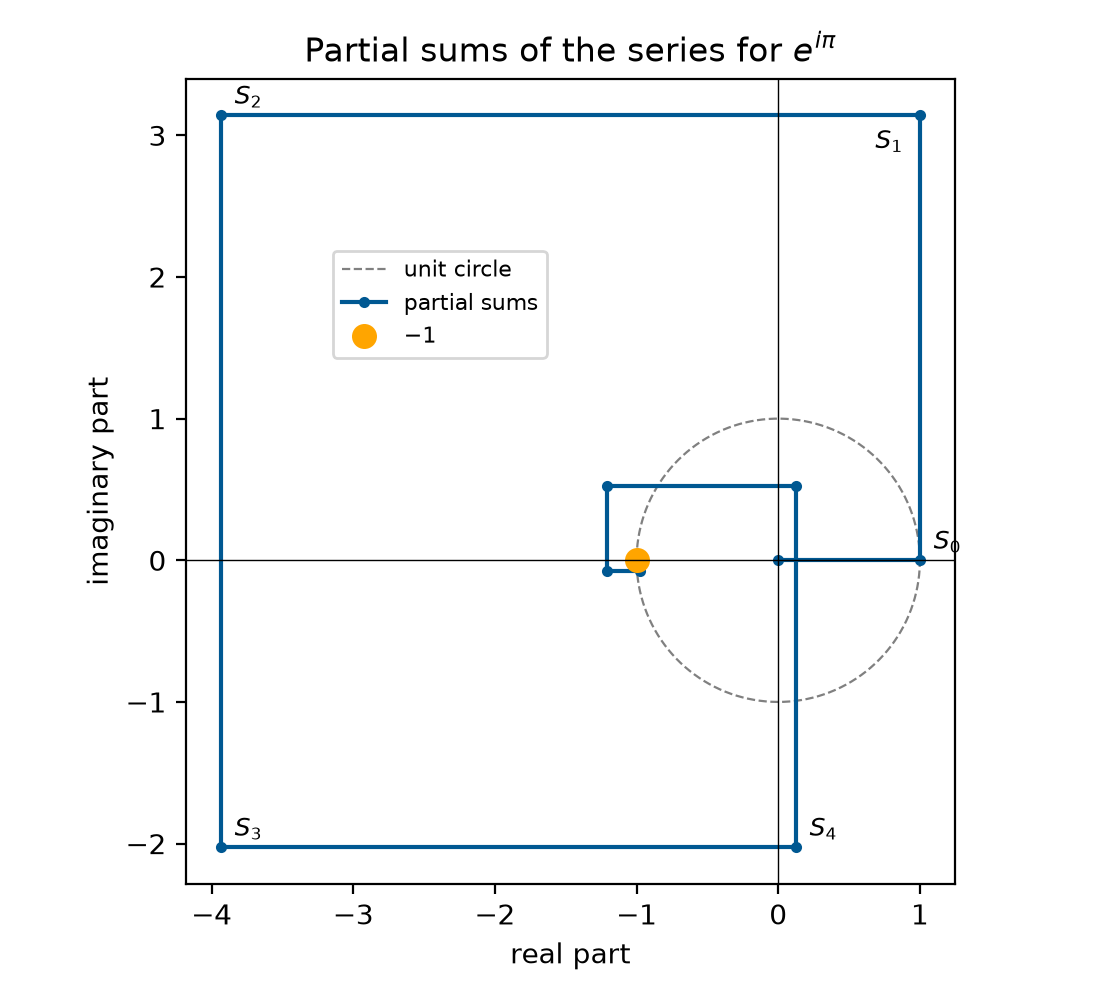
\includegraphics[width=0.6\textwidth]{partial_sums.png}
\caption{Each partial sum turns a corner, and the path spirals in on $-1$.}
\label{fig:euler-partial-sums}
\end{figure}

The path spirals in on $-1 + 0i$. So $e^{i\pi} = -1$, which is Euler's identity,
$e^{i\pi} + 1 = 0$.

\section{A Point on the Unit Circle}\index{unit circle}
In the Trigonometric Functions chapter, $(\cos\theta, \sin\theta)$ was the point on
the unit circle at angle $\theta$. In the complex plane, the point $(a, b)$ is the
number $a + bi$. So Euler's formula says:

\begin{center}
\emph{$e^{i\theta}$ is the point on the unit circle at angle $\theta$.}
\end{center}

\begin{figure}[H]
\centering
\begin{tikzpicture}[scale=2.2]
\draw[-latex] (-1.3,0) -- (1.5,0) node[above] {real};
\draw[-latex] (0,-1.3) -- (0,1.35) node[above] {imaginary};
\draw[gray] (0,0) circle (1);
\draw[thick, sdkblue, -latex] (0,0) -- (50:1);
\fill[sdkblue] (50:1) circle (0.03) node[above right] {$e^{i\theta} = \cos\theta + i\sin\theta$};
\draw[dashed] (50:1) -- ({cos(50)},0) node[below] {$\cos\theta$};
\draw[dashed] (50:1) -- (0,{sin(50)}) node[left] {$\sin\theta$};
\draw (0.3,0) arc (0:50:0.3); \node at (25:0.42) {$\theta$};
\fill (1,0) circle (0.025) node[below right] {$e^{0} = 1$};
\fill (0,1) circle (0.025) node[above left] {$e^{i\pi/2} = i$};
\fill (-1,0) circle (0.025) node[below left] {$e^{i\pi} = -1$};
\fill (0,-1) circle (0.025) node[below right] {$e^{i3\pi/2} = -i$};
\end{tikzpicture}
\caption{As $\theta$ increases, $e^{i\theta}$ travels counterclockwise around the unit circle.}
\label{fig:euler-circle}
\end{figure}

As $\theta$ goes from 0 to $2\pi$, $e^{i\theta}$ walks once around the circle. Some
landmarks:
$$e^{0} = 1, \qquad e^{i\pi/2} = i, \qquad e^{i\pi} = -1, \qquad e^{i3\pi/2} = -i, \qquad e^{2\pi i} = 1$$
Euler's identity is no longer mysterious: walk halfway around the unit circle, and
you land on $-1$. Because every point of the circle is at distance 1 from 0,
$$\left|e^{i\theta}\right| = \sqrt{\cos^2\theta + \sin^2\theta} = 1$$

\begin{Exercise}[title={Around the Circle}, label=eu_values]
Write each number in the form $a + bi$.
\begin{enumerate}
\item $e^{i\pi/3}$
\item $e^{i\pi/4}$
\item $e^{i3\pi/2}$
\item $e^{10\pi i}$
\end{enumerate}
\end{Exercise}
\begin{Answer}[ref=eu_values]
\begin{enumerate}
\item $\cos\frac{\pi}{3} + i\sin\frac{\pi}{3} = \frac{1}{2} + \frac{\sqrt{3}}{2}i$
\item $\frac{\sqrt{2}}{2} + \frac{\sqrt{2}}{2}i$
\item $\cos\frac{3\pi}{2} + i\sin\frac{3\pi}{2} = -i$
\item $10\pi$ is five full turns, so $e^{10\pi i} = 1$.
\end{enumerate}
\end{Answer}

\section{Polar Form}\index{complex number!polar form}
Every point in the plane can be described by its distance $r$ from the origin and
its angle $\theta$, as in the Polar Coordinates chapter. For a complex number, that
means
$$z = a + bi = r(\cos\theta + i\sin\theta) = re^{i\theta}$$
This is the \newterm{polar form} of $z$. The distance $r = |z| = \sqrt{a^2 + b^2}$ is
the \newterm{modulus}, and the angle $\theta$ is the \newterm{argument}. As with
polar coordinates, find $\theta$ from $\tan\theta = \frac{b}{a}$, and check which
quadrant the point is in.

For example, $1 + i$ is at distance $\sqrt{2}$ and angle $\frac{\pi}{4}$, so
$1 + i = \sqrt{2}\,e^{i\pi/4}$. And $-2 = 2e^{i\pi}$.

\subsection{Multiplying: Stretch and Rotate}
The Complex Numbers chapter claimed that multiplying by a complex number rotates
and stretches. Polar form shows exactly how. Using the exponent rule,
$$\left(r_1 e^{i\theta_1}\right)\left(r_2 e^{i\theta_2}\right) = r_1 r_2\, e^{i(\theta_1 + \theta_2)}$$
\begin{center}
\emph{To multiply complex numbers, multiply their lengths and add their angles.}
\end{center}
Multiplying by $i = e^{i\pi/2}$ keeps the length (it is 1) and adds $90^\circ$ to
the angle: a quarter turn, just as you saw before.

\textbf{Example}: Multiply $(1 + i)(\sqrt{3} + i)$ using polar form.

\textbf{Solution}: $1 + i = \sqrt{2}\,e^{i\pi/4}$ and $\sqrt{3} + i = 2e^{i\pi/6}$. So the
product has length $2\sqrt{2} \approx 2.83$ and angle
$\frac{\pi}{4} + \frac{\pi}{6} = \frac{5\pi}{12}$, which is $75^\circ$. Check by
multiplying the ordinary way: $(1 + i)(\sqrt{3} + i) = (\sqrt{3} - 1) + (\sqrt{3} + 1)i
\approx 0.732 + 2.732i$, whose length is $\sqrt{0.536 + 7.464} = \sqrt{8} = 2\sqrt{2}$.

\subsection{Powers: De Moivre's Formula}\index{De Moivre's formula}
Multiplying a number by itself $n$ times multiplies its length $n$ times and adds
its angle $n$ times:
$$\left(re^{i\theta}\right)^n = r^n e^{in\theta}$$
This is \newterm{De Moivre's formula}. It turns big powers into easy ones.

\textbf{Example}: Find $(1 + i)^{10}$.

\textbf{Solution}: $(1 + i)^{10} = \left(\sqrt{2}\,e^{i\pi/4}\right)^{10} = (\sqrt{2})^{10}\, e^{i10\pi/4} = 32\, e^{i5\pi/2}$.
An angle of $\frac{5\pi}{2}$ is one full turn plus $\frac{\pi}{2}$, so
$(1 + i)^{10} = 32i$. Doing this by expanding would take a long time.

\subsection{Roots of Unity}\index{roots of unity}
How many numbers satisfy $z^3 = 1$? The real number 1 does, but the Fundamental
Theorem of Algebra promises three solutions. Write $z = e^{i\theta}$. Then
$z^3 = e^{i3\theta}$, which equals 1 whenever $3\theta$ is a whole number of turns:
$3\theta = 0, 2\pi, 4\pi$. So the three \newterm{cube roots of unity} are
$$1, \qquad e^{i2\pi/3} = -\frac{1}{2} + \frac{\sqrt{3}}{2}i, \qquad e^{i4\pi/3} = -\frac{1}{2} - \frac{\sqrt{3}}{2}i$$
In general, the $n$ solutions of $z^n = 1$ are $e^{i2\pi k/n}$ for $k = 0, 1, \dots, n-1$.
They sit evenly spaced around the unit circle, at the corners of a regular
$n$-sided polygon.

\begin{figure}[H]
\centering
\begin{tikzpicture}[scale=1.6]
\draw[-latex] (-1.4,0) -- (1.5,0);
\draw[-latex] (0,-1.3) -- (0,1.35);
\draw[gray] (0,0) circle (1);
\draw[thick, sdkblue] (0:1) -- (120:1) -- (240:1) -- cycle;
\foreach \a/\l/\p in {0/1/above right, 120/{e^{i2\pi/3}}/above left, 240/{e^{i4\pi/3}}/below left}
  \fill[sdkblue] (\a:1) circle (0.04) node[\p] {$\l$};
\end{tikzpicture}
\caption{The three cube roots of 1 form an equilateral triangle.}
\label{fig:cube-roots}
\end{figure}

\begin{Exercise}[title={Polar Form}, label=eu_polar]
\begin{enumerate}
\item Write $-3 + 3i$ in polar form.
\item Use polar form to find $(1 - \sqrt{3}i)^6$.
\item Find all three cube roots of 8.
\end{enumerate}
\end{Exercise}
\begin{Answer}[ref=eu_polar]
\begin{enumerate}
\item $r = \sqrt{9 + 9} = 3\sqrt{2}$. The point is in the second quadrant at angle
$\frac{3\pi}{4}$ ($135^\circ$), so $-3 + 3i = 3\sqrt{2}\,e^{i3\pi/4}$.
\item $1 - \sqrt{3}i = 2e^{-i\pi/3}$, so $(1 - \sqrt{3}i)^6 = 2^6 e^{-i2\pi} = 64$.
\item Each cube root has length $\sqrt[3]{8} = 2$, and the angles are spaced by
$\frac{2\pi}{3}$: $2$, $2e^{i2\pi/3} = -1 + \sqrt{3}i$, and $2e^{i4\pi/3} = -1 - \sqrt{3}i$.
\end{enumerate}
\end{Answer}

\section{Trigonometry for Free}\index{trigonometric identities!from Euler's formula}
In the Trigonometric Identities chapter, the sum formulas took a careful geometric
proof. Euler's formula gives them in two lines. Start with
$e^{i(a+b)} = e^{ia}e^{ib}$ and expand both sides:
\begin{align*}
\cos(a+b) + i\sin(a+b) &= (\cos a + i\sin a)(\cos b + i\sin b) \\
&= (\cos a\cos b - \sin a\sin b) + i(\sin a\cos b + \cos a\sin b)
\end{align*}
Two complex numbers are equal only when their real parts match and their imaginary
parts match:
$$\cos(a+b) = \cos a\cos b - \sin a\sin b, \qquad \sin(a+b) = \sin a\cos b + \cos a\sin b$$
You never need to memorize these again; you can rebuild them whenever you want.

Euler's formula also runs backward. Since $e^{-i\theta} = \cos\theta - i\sin\theta$,
adding and subtracting gives
$$\cos\theta = \frac{e^{i\theta} + e^{-i\theta}}{2}, \qquad \sin\theta = \frac{e^{i\theta} - e^{-i\theta}}{2i}$$
so every trig function is secretly made of exponentials.

\begin{Exercise}[title={Double Angles}, label=eu_double]
Use $e^{i2\theta} = \left(e^{i\theta}\right)^2$ to find formulas for $\cos 2\theta$ and
$\sin 2\theta$.
\end{Exercise}
\begin{Answer}[ref=eu_double]
$\cos 2\theta + i\sin 2\theta = (\cos\theta + i\sin\theta)^2 = \cos^2\theta - \sin^2\theta + 2i\sin\theta\cos\theta$.
Matching parts: $\cos 2\theta = \cos^2\theta - \sin^2\theta$ and $\sin 2\theta = 2\sin\theta\cos\theta$.
\end{Answer}

\section{Spinning and Oscillating}

Now let the angle grow with time: $z(t) = e^{i\omega t}$ is a point going around the
unit circle with angular speed $\omega$. Differentiating each part,
$$\frac{d}{dt}e^{i\omega t} = \frac{d}{dt}\left(\cos\omega t + i\sin\omega t\right) = -\omega\sin\omega t + i\omega\cos\omega t = i\omega\left(\cos\omega t + i\sin\omega t\right) = i\omega\, e^{i\omega t}$$
So the usual rule $\frac{d}{dt}e^{kt} = ke^{kt}$ still works with $k = i\omega$. And it
has a picture: the velocity is the position multiplied by $i\omega$, that is, rotated
$90^\circ$ and stretched by $\omega$. The velocity of circular motion is always
tangent to the circle, just as you saw in the Circular Motion chapter.

Differentiate again: $\frac{d^2}{dt^2}e^{i\omega t} = (i\omega)^2 e^{i\omega t} = -\omega^2 e^{i\omega t}$.
That is the equation of a spring, $x'' = -\omega^2 x$. Its real part, $\cos\omega t$,
is the spring's back-and-forth motion: a mass on a spring is the shadow of a point
going around a circle.

\subsection{Damped Oscillations}\index{damping!complex exponential}
In the Differential Equations chapter, a damped spring had characteristic roots
$r = \alpha \pm i\beta$, and the table claimed the motion was
$e^{\alpha t}(C_1\cos\beta t + C_2\sin\beta t)$. Now you can see why. The guess
$e^{rt}$ with $r = \alpha + i\beta$ gives
$$e^{(\alpha + i\beta)t} = e^{\alpha t}e^{i\beta t} = e^{\alpha t}\left(\cos\beta t + i\sin\beta t\right)$$
The factor $e^{\alpha t}$ (with $\alpha < 0$) shrinks the swing, and the
$e^{i\beta t}$ part spins, producing the oscillation. A complex root is just an
exponential that rotates while it decays.

\subsection{Alternating Current}\index{phasor}
Electrical engineers use this idea every day. They write an AC voltage
$V_0\cos\omega t$ as the real part of $V_0e^{i\omega t}$, a rotating arrow called a
\newterm{phasor}. Since differentiating just multiplies by $i\omega$, the calculus in a
circuit with capacitors and inductors turns into ordinary algebra with complex
numbers.

\section{Complex Exponentials in Python}
Python writes $i$ as \mintinline{python}{1j}. The \mintinline{python}{cmath} library
has complex versions of the math functions, plus tools for polar form:
\begin{minted}{python}
import cmath, math

print(cmath.exp(1j * math.pi))         # e^(i pi)
print(cmath.polar(1 + 1j))             # (r, theta) for 1 + i
print(cmath.rect(2, math.pi / 3))      # 2 e^(i pi/3) back to a + bi
print((1 + 1j) ** 10)                  # De Moivre says 32i
\end{minted}
\begin{verbatim}
(-1+1.2246467991473532e-16j)
(1.4142135623730951, 0.7853981633974483)
(1.0000000000000002+1.7320508075688772j)
32j
\end{verbatim}
The first answer should be exactly $-1$. The tiny imaginary part, about
$10^{-16}$, is rounding error: the computer's value of $\pi$ is very close to $\pi$,
but not exact.

\begin{Exercise}[title={The Strangest Power}, label=eu_ii]
Use $i = e^{i\pi/2}$ to compute $i^i$. Is the answer real or imaginary?
\end{Exercise}
\begin{Answer}[ref=eu_ii]
$i^i = \left(e^{i\pi/2}\right)^i = e^{i \cdot i\pi/2} = e^{-\pi/2} \approx 0.2079$. An imaginary
number raised to an imaginary power is a real number! (Because $i$ is also
$e^{i(\pi/2 + 2\pi k)}$ for any whole number $k$, $i^i$ has other values too, such as
$e^{-5\pi/2}$; $e^{-\pi/2}$ is the standard one, and it is what Python's
\mintinline{python}{1j ** 1j} returns.)
\end{Answer}

\begin{Exercise}[title={Conjugates on the Circle}, label=eu_conj]
Show that $e^{-i\theta}$ is the complex conjugate of $e^{i\theta}$, and that their
product is 1. What does this mean geometrically?
\end{Exercise}
\begin{Answer}[ref=eu_conj]
$e^{-i\theta} = \cos(-\theta) + i\sin(-\theta) = \cos\theta - i\sin\theta$, which is the
conjugate of $\cos\theta + i\sin\theta$. Their product is
$e^{i\theta}e^{-i\theta} = e^{0} = 1$ (or, directly, $\cos^2\theta + \sin^2\theta = 1$).
Geometrically, $e^{-i\theta}$ is the reflection of $e^{i\theta}$ across the real axis,
and rotating by $\theta$ and then by $-\theta$ brings you back to 1.
\end{Answer}

\begin{Exercise}[title={Check Euler with Python}, label=eu_python]
Write a short Python program that checks Euler's formula for
$\theta = 0, 0.5, 1, 1.5, \dots, 3$ by printing the difference between
\mintinline{python}{cmath.exp(1j * theta)} and
\mintinline{python}{math.cos(theta) + 1j * math.sin(theta)}.
\end{Exercise}
\begin{Answer}[ref=eu_python]
\begin{minted}{python}
import cmath, math

for k in range(7):
    theta = 0.5 * k
    lhs = cmath.exp(1j * theta)
    rhs = math.cos(theta) + 1j * math.sin(theta)
    print(theta, abs(lhs - rhs))
\end{minted}
Every difference is 0 or a rounding error around $10^{-16}$.
\end{Answer}
